\section{Results}\label{sec:results}

\subsection{Overall performance (RQ1)}\label{sec:res-main}
Table~\ref{tab:main} reports all models on the test periods and Fig.~\ref{fig:pr} shows the precision--recall curves of the ensemble and its members.

\begin{table*}[t]
\caption{Positive-class results on the test period. Thresholds come from validation data only; the 50-tree Random Forest uses 0.5 as in prior work. Brackets give 95\% bootstrap intervals for the ensemble.}\label{tab:main}
\centering
\begin{tabular}{llrrrrrr}
\toprule
Layer & Model & Precision & Recall & F1 & MCC & PR-AUC & ROC-AUC \\
\midrule
Transactions & Logistic regression & 0.895 & 0.519 & 0.657 & 0.666 & 0.718 & 0.894 \\
 & Isolation Forest (unsupervised) & 0.064 & 0.989 & 0.121 & $-$0.086 & 0.036 & 0.168 \\
 & Random Forest, 50 trees~\cite{elmougy2023} & 0.959 & 0.719 & 0.822 & 0.821 & 0.783 & 0.913 \\
 & LightGBM & 0.952 & 0.731 & 0.827 & 0.825 & 0.808 & 0.938 \\
 & XGBoost & 0.885 & 0.734 & 0.803 & 0.794 & 0.812 & 0.945 \\
 & Random Forest & 0.961 & 0.714 & 0.819 & 0.819 & 0.801 & 0.941 \\
 & \textbf{Ensemble} & \textbf{0.961} & \textbf{0.729} & \textbf{0.829} & \textbf{0.828} & \textbf{0.806} & \textbf{0.942} \\
 & & [0.947, 0.974] & [0.704, 0.758] & [0.811, 0.850] & [0.811, 0.848] & [0.783, 0.827] & [0.935, 0.949] \\
\midrule
Wallets & Logistic regression & 0.354 & 0.403 & 0.376 & 0.340 & 0.264 & 0.810 \\
 & Isolation Forest (unsupervised) & 0.055 & 0.948 & 0.104 & 0.032 & 0.061 & 0.552 \\
 & Random Forest, 50 trees~\cite{elmougy2023} & 0.381 & 0.187 & 0.250 & 0.239 & 0.298 & 0.856 \\
 & LightGBM & 0.957 & 0.560 & 0.707 & 0.722 & 0.721 & 0.937 \\
 & XGBoost & 0.928 & 0.502 & 0.651 & 0.671 & 0.704 & 0.934 \\
 & Random Forest & 0.940 & 0.519 & 0.669 & 0.687 & 0.701 & 0.933 \\
 & \textbf{Ensemble} & \textbf{0.908} & \textbf{0.583} & \textbf{0.710} & \textbf{0.716} & \textbf{0.721} & \textbf{0.937} \\
 & & [0.898, 0.917] & [0.570, 0.596] & [0.699, 0.721] & [0.706, 0.726] & [0.709, 0.730] & [0.934, 0.940] \\
\midrule
Network & Logistic regression & 0.080 & 0.520 & 0.139 & 0.200 & 0.072 & 0.931 \\
 & Isolation Forest (unsupervised) & 0.214 & 0.073 & 0.109 & 0.124 & 0.045 & 0.836 \\
 & Random Forest, 50 trees & 0.836 & 0.139 & 0.239 & 0.341 & 0.751 & 0.959 \\
 & LightGBM & 0.671 & 0.549 & 0.604 & 0.606 & 0.554 & 0.975 \\
 & XGBoost & 0.836 & 0.492 & 0.619 & 0.641 & 0.618 & 0.972 \\
 & Random Forest & 0.253 & 0.124 & 0.166 & 0.175 & 0.187 & 0.972 \\
 & \textbf{Ensemble} & \textbf{0.886} & \textbf{0.466} & \textbf{0.610} & \textbf{0.642} & \textbf{0.522} & \textbf{0.976} \\
 & & [0.855, 0.918] & [0.431, 0.501] & [0.575, 0.643] & [0.611, 0.671] & [0.491, 0.551] & [0.969, 0.982] \\
\bottomrule
\end{tabular}
\tablenote{Reference models (first three rows of each block) use the original features; ensemble members use all features. The wallet and transaction ensembles and their members include graph-derived features.}
\end{table*}

\begin{figure*}[t]
\centering
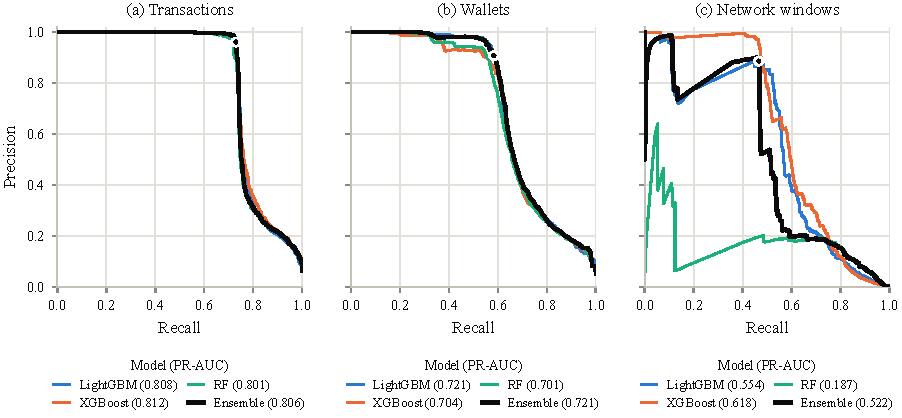
\includegraphics[width=\textwidth]{figures/fig_pr_curves.pdf}
\caption{Precision--recall curves on the test period for the ensemble and its members. The dot marks the operating point fixed on validation data. In (a) all curves fall sharply near recall 0.73: about a quarter of the illicit transactions are ranked no better than licit ones. In (c) the ensemble is pulled below its best member by a Random Forest member that ranks poorly.}\label{fig:pr}
\end{figure*}

Three observations follow. First, precision is high and recall is the limiting factor in every layer: the ensemble is rarely wrong when it flags an entity (precision 0.96, 0.91 and 0.89) but misses 27\%, 42\% and 53\% of the positives. Second, the ensemble is not uniformly the best model. It has the highest F1 for transactions and wallets, by small margins over LightGBM, and for network windows it is slightly below XGBoost in F1 and clearly below it in PR-AUC. Averaging protects against a weak member only if no member is very weak; the network Random Forest (PR-AUC 0.187) is, and it lowers the average. Third, the plain 50-tree Random Forest behaves very differently across layers: it is nearly as good as the ensemble on transactions, far worse on wallets, and on network windows it has the best PR-AUC of all models (0.751) while its fixed threshold of 0.5 yields a recall of 0.14.

\subsection{Comparison with published results}\label{sec:res-published}
Table~\ref{tab:published} sets our numbers beside those of Elmougy and Liu~\cite{elmougy2023}, who use the same train and test time steps.

\begin{table}[t]
\caption{Illicit-class results against prior work on Elliptic++ (train steps 1--34, test steps 35--49)}\label{tab:published}
\centering
\setlength{\tabcolsep}{3pt}
\begin{tabular}{lrrr}
\toprule
Model & Precision & Recall & F1 \\
\midrule
\multicolumn{4}{l}{\emph{Transactions}} \\
Published RF~\cite{elmougy2023} & 0.975 & 0.719 & 0.828 \\
Published XGBoost~\cite{elmougy2023} & 0.793 & 0.718 & 0.754 \\
Published RF+MLP+XGB~\cite{elmougy2023} & 0.962 & 0.723 & 0.826 \\
Reproduced RF (ours) & 0.959 & 0.719 & 0.822 \\
Ensemble (ours) & 0.961 & 0.729 & 0.829 \\
\midrule
\multicolumn{4}{l}{\emph{Wallets}} \\
Published RF~\cite{elmougy2023} & 0.911 & 0.789 & 0.845 \\
Published XGBoost~\cite{elmougy2023} & 0.869 & 0.534 & 0.662 \\
Published RF+MLP+XGB~\cite{elmougy2023} & 0.933 & 0.572 & 0.709 \\
Reproduced RF, one row per wallet & 0.381 & 0.187 & 0.250 \\
Reproduced RF, rows as distributed & 0.525 & 0.306 & 0.387 \\
Ensemble (ours), one row per wallet & 0.908 & 0.583 & 0.710 \\
Ensemble (ours), row per appearance & 0.909 & 0.573 & 0.702 \\
\bottomrule
\end{tabular}
\tablenote{Published values are copied from Tables 7 and 8 of~\cite{elmougy2023} (arXiv version 1). ``Rows as distributed'' uses the released file including duplicate rows and the time step as a feature.}
\end{table}

\emph{Transactions.} The published Random Forest is reproduced closely (F1 0.822 against 0.828; identical recall). Our ensemble reaches 0.829. A paired bootstrap on the test set gives a difference between the ensemble and the reproduced forest of $+0.007$ F1 with a 95\% interval of $[-0.0001,\, 0.0145]$; the two models disagree on 56 of 16,670 test transactions. We therefore claim parity with the best published result, not an improvement.

\emph{Wallets.} The published wallet result is not reproduced under any time-ordered split that we tried. The same model configuration yields F1 0.250 with one row per wallet and 0.387 on the rows as distributed, against the published 0.845. Section~\ref{sec:res-split} shows that a random split of the same data gives values close to the published one. Within our protocol the ensemble reaches 0.710, close to the published three-model ensemble (0.709), but since the single-model figures cannot be reconciled we do not regard the two as measurements of the same task.

\subsection{What graph features contribute (RQ2)}\label{sec:res-graph}

\begin{table}[t]
\caption{Effect of graph-derived features on the ensemble (test period)}\label{tab:graph}
\centering
\setlength{\tabcolsep}{3pt}
\begin{tabular}{llrrrr}
\toprule
Layer & Features & Prec. & Recall & F1 & PR-AUC \\
\midrule
Transactions & original (182) & 0.911 & 0.731 & 0.811 & 0.800 \\
 & with graph (555) & 0.961 & 0.729 & 0.829 & 0.806 \\
\midrule
Wallets & original (55) & 0.634 & 0.249 & 0.357 & 0.426 \\
 & with graph (174) & 0.908 & 0.583 & 0.710 & 0.721 \\
\bottomrule
\end{tabular}
\end{table}

\begin{figure}[t]
\centering
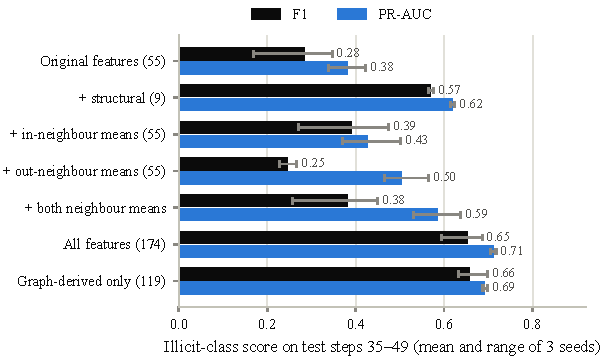
\includegraphics[width=\linewidth]{figures/fig_wallet_ablation.pdf}
\caption{Wallet layer, single LightGBM: contribution of feature groups. Bars are means over three seeds and whiskers show the range. Nine structural descriptors account for most of the gain, and graph-derived features alone perform as well as all features together.}\label{fig:ablation}
\end{figure}

Table~\ref{tab:graph} shows the central asymmetry of this study. At the transaction level, graph-derived features change little: F1 rises by 0.018, entirely through fewer false positives (77 to 32), and PR-AUC by 0.006. At the wallet level they double F1 (0.357 to 0.710) and raise PR-AUC from 0.426 to 0.721.

\subsubsection{Which features matter} Fig.~\ref{fig:ablation} decomposes the wallet gain with a single LightGBM. Adding only the nine structural descriptors raises PR-AUC from 0.38 to 0.62. Neighbour means help less on their own and are unstable across seeds, but combine with the structural descriptors to reach 0.71. Most strikingly, the 119 graph-derived features \emph{without} the original wallet features reach PR-AUC 0.69 and F1 0.66, the same as all 174 features. At this level, where a wallet sits in the interaction graph and what its counterparties look like is more informative than its own behavioural summary.

\subsubsection{Why the two levels differ} Two facts explain the asymmetry. The first is that the transaction features already contain neighbourhood information: 72 of the Elliptic features are aggregates over one-hop neighbours~\cite{weber2019}, so~\eqref{eq:mean} largely repeats what is present. The second is label homophily~\cite{mcpherson2001}, summarised in Table~\ref{tab:homophily}. In the address graph, a labelled neighbour of an illicit wallet is itself illicit in 76\% of cases, against a base rate of 5.4\%; in the transaction graph the corresponding figure is 54\% against 9.8\%. Illicit wallets form tighter neighbourhoods than illicit transactions do, which is what one would expect if several addresses take part in the same illicit transaction.

\begin{table}[t]
\caption{Label agreement along edges whose endpoints are both labelled}\label{tab:homophily}
\centering
\setlength{\tabcolsep}{3pt}
\begin{tabular}{lrr}
\toprule
 & Tx graph & Address graph \\
\midrule
Edges with both ends labelled & 36,624 & 1,091,809 \\
Illicit base rate, labelled nodes & 0.098 & 0.054 \\
P(nbr. illicit $|$ node illicit) & 0.541 & 0.764 \\
P(nbr. illicit $|$ node licit) & 0.024 & 0.004 \\
\bottomrule
\end{tabular}
\tablenote{Descriptive statistics over all labelled nodes; labels are never used as model inputs.}
\end{table}

\subsubsection{Does the gain depend on look-ahead?} For transactions the question does not arise: none of the 234,355 edges connects transactions of different time steps, so the neighbourhood of a transaction is contemporaneous. For wallets, 542,145 of the 2,775,637 edges connect wallets with different first-appearance steps, and 80,617 cross the boundary between training and test periods. The exposure of the training set is small: 0.7\% of labelled training wallets have a neighbour that first appears in the test period. Restricting every aggregation to the causal neighbourhood~\eqref{eq:causal} leaves ranking quality essentially unchanged: with a single LightGBM on the original features, degrees and neighbour means, PR-AUC is 0.690 (range over three seeds 0.679--0.700) with causal neighbourhoods and 0.698 (0.695--0.702) with all neighbours, and the oracle F1 is 0.690 against 0.701.
The wallet gain is therefore not an artefact of adjacency to future wallets, in contrast to the graph-network setting examined in~\cite{maganti2026}. The look-ahead that remains lies in the wallet features themselves (Section~\ref{sec:data-wallets}). Its reach is limited as well: 98.4\% of test wallets (and 92.3\% of training wallets) are active in exactly one time step, so that their lifetime aggregates cannot contain later activity; on this subset the ensemble's F1 is 0.715, against 0.710 overall. The 1,434 test wallets active in several steps are the ones the model fails on (48 illicit, one detected).

\subsection{The split decides the result (RQ3)}\label{sec:res-split}

\begin{table}[t]
\caption{Temporal against random splits (threshold 0.5; random splits: mean of three seeds)}\label{tab:split}
\centering
\setlength{\tabcolsep}{3pt}
\begin{tabular}{llrrr}
\toprule
Rows & Model & \multicolumn{1}{c}{Temporal} & \multicolumn{1}{c}{Random} & \multicolumn{1}{c}{Gap} \\
 & & \multicolumn{1}{c}{F1} & \multicolumn{1}{c}{F1} & \\
\midrule
Transactions & RF-50, original & 0.822 & 0.939 & +0.117 \\
 & LightGBM, all & 0.829 & 0.957 & +0.128 \\
\midrule
Wallets, 1 row each & RF-50, original & 0.250 & 0.869 & +0.619 \\
 & LightGBM, all & 0.599 & 0.906 & +0.307 \\
\midrule
Wallets, as distrib. & RF-50, orig.+step & 0.387 & 0.955 & +0.568 \\
\bottomrule
\end{tabular}
\tablenote{Standard deviations over random-split seeds are at most 0.006. In the random split of the distributed wallet rows, 34.8\% of test rows belong to a wallet that also has a row in the training part (6.1\% under the temporal split).}
\end{table}

Table~\ref{tab:split} repeats the same models under a stratified random 70/30 split. For transactions a random split adds about 0.12 F1. For wallets the effect is far larger: the 50-tree Random Forest moves from 0.250 to 0.869 with one row per wallet and to 0.955 on the rows as distributed, where a third of the test rows have a twin with identical features and label in the training part.

Two points deserve emphasis. First, the published wallet figure (precision 0.911, recall 0.789, F1 0.845) lies close to our random-split result with one row per wallet (0.965, 0.790, 0.869) and far from every temporal result. We cannot determine from the paper how its rows were assigned, and we do not claim that a random split was used; the observation is only that we can approach the published value with a split that is not time-ordered and cannot with one that is. Second, the gap is not specific to duplicated rows. Even with one row per wallet, random assignment mixes wallets of the same time step, and often of the same transaction, across the two sides, and the homophily documented in Table~\ref{tab:homophily} makes such neighbours near-copies of one another. A random split therefore measures interpolation within an episode of activity, while a temporal split measures transfer to later episodes; only the latter corresponds to deployment~\cite{pendlebury2019,arp2022}.

\subsection{Stability over time (RQ4)}\label{sec:res-drift}

\begin{figure}[t]
\centering
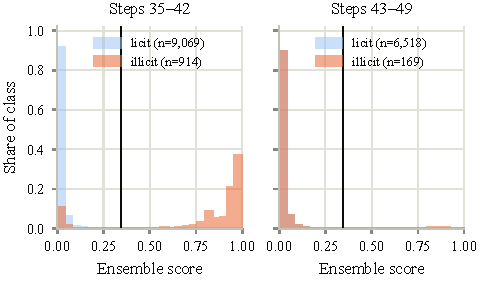
\includegraphics[width=\linewidth]{figures/fig_tx_scores.pdf}
\caption{Ensemble scores of test transactions by true class, before and after the dark-market shutdown at step 43. The vertical line is the decision threshold. After the shutdown, illicit transactions receive the same scores as licit ones.}\label{fig:scores}
\end{figure}

\begin{figure}[t]
\centering
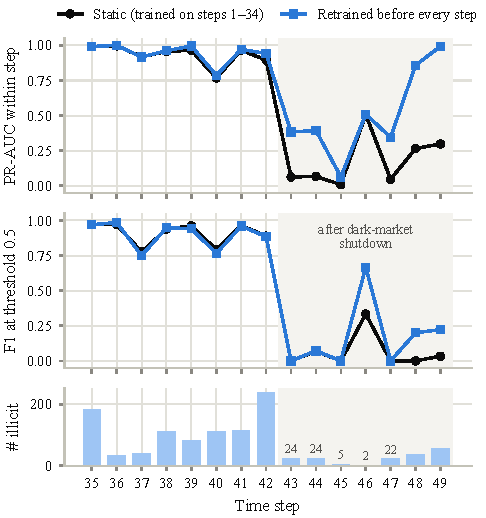
\includegraphics[width=\linewidth]{figures/fig_tx_drift.pdf}
\caption{Transactions, single LightGBM, per test step. Retraining before every step restores ranking quality within a few steps of the shutdown (top) but hardly improves decisions at a fixed threshold (middle). Steps 43--47 contain between 2 and 24 illicit transactions each (bottom), so per-step values there are noisy.}\label{fig:drift}
\end{figure}

\begin{table}[t]
\caption{Static against retrained models by period (single LightGBM, threshold 0.5)}\label{tab:drift}
\centering
\setlength{\tabcolsep}{3pt}
\begin{tabular}{lllrrrr}
\toprule
Layer & Steps & Model & F1 & PR-AUC & ROC & Oracle \\
\midrule
Transact. & 35--42 & static & 0.917 & 0.924 & 0.975 & 0.918 \\
 & & retrained & 0.911 & 0.939 & 0.984 & 0.920 \\
 & 43--49 & static & 0.032 & 0.062 & 0.766 & 0.115 \\
 & & retrained & 0.140 & 0.616 & 0.967 & 0.650 \\
\midrule
Wallets & 35--42 & static & 0.773 & 0.833 & 0.962 & 0.801 \\
 & & retrained & 0.742 & 0.849 & 0.961 & 0.817 \\
 & 43--49 & static & 0.289 & 0.504 & 0.910 & 0.528 \\
 & & retrained & 0.469 & 0.605 & 0.955 & 0.543 \\
\bottomrule
\end{tabular}
\tablenote{Scores are pooled over the steps of a period. Retraining uses all labels up to the previous step. Oracle F1 is the best F1 any single threshold could give on that period and is an upper bound.}
\end{table}

\subsubsection{The static model fails by ranking, not by threshold} The transaction ensemble achieves F1 0.918 on steps 35--42 and 0.031 on steps 43--49, where it detects 3 of 169 illicit transactions. Fig.~\ref{fig:scores} shows why: after step 43 almost all illicit transactions receive scores near zero, as licit ones do (PR-AUC 0.062 at a prevalence of 0.025; for the static LightGBM of Table~\ref{tab:drift}, 97\% of them score below 0.05). No threshold repairs this; the best possible F1 on steps 43--49 is 0.112. Over the whole test period the validation-selected threshold costs only 0.003 F1 relative to the oracle. The step-43 event, attributed in~\cite{weber2019} to the closure of a dark market, removed the kind of illicit activity the model had learned; the illicit transactions that remain are of a kind it had not seen.

\subsubsection{Retraining restores ranking, then the threshold becomes the problem} Table~\ref{tab:drift} and Fig.~\ref{fig:drift} compare the static model with one retrained before every step. On steps 43--49 retraining lifts PR-AUC from 0.062 to 0.616 and ROC-AUC from 0.766 to 0.967; by steps 48 and 49 the per-step PR-AUC is 0.86 and 0.99. The F1 at the fixed threshold, however, only rises from 0.032 to 0.140, while the oracle F1 is 0.650. The retrained model ranks the new illicit transactions correctly but assigns them scores below 0.5, because they are still a small minority of its training data.

This reconciles our observation with that of Bhatt and Sharma~\cite{bhatt2026}, who attribute losses under non-stationarity to miscalibrated decision rules. Both mechanisms occur, in sequence: a model that is never updated loses the ranking itself, and a model that is updated recovers the ranking but needs its threshold re-estimated. Reporting only a threshold metric would hide the recovery, and reporting only a ranking metric would hide that decisions remain poor.

\subsubsection{Wallets} Drift at the wallet level is milder and less regular. The ensemble's F1 is 0.802 on steps 35--42 and 0.569 on steps 43--49, with per-step values between 0.01 and 0.97. Retraining helps after the shutdown (PR-AUC 0.504 to 0.605) and again exposes threshold instability: at step 37 the retrained model has PR-AUC 0.91 but F1 0.14 at threshold 0.5, against 0.78 for the static model.

\subsubsection{What the drift is not} We attempted to quantify the shift with a domain classifier that separates illicit transactions of two periods. Its cross-validated ROC-AUC is 1.000 for every pair of periods, including a control pair inside the training period (steps 1--17 against 18--34), and for licit transactions as well. The features of Elliptic thus identify the period of a transaction perfectly, which makes this diagnostic uninformative about the shutdown specifically. It also means that covariate shift is present between any two periods, and that a model can in principle recognise the period of a test point; under a random split this is a further channel through which results are inflated.

\subsection{Unsupervised detection}\label{sec:res-unsup}
Isolation Forest, fitted on licit training transactions, attains a ROC-AUC of 0.168 on the test period, well below chance. The inversion is systematic: it is 0.107 on the labelled training period and 0.110 on steps 35--42, and returns to chance (0.483) after the shutdown. Illicit transactions are, by the isolation criterion, \emph{more} typical than licit ones, so that in this data ``illicit'' and ``anomalous'' are different properties before step 43 and unrelated ones after it. On wallets the detector is at chance (0.552); on network windows it has some ranking ability (0.836) but poor precision (PR-AUC 0.045 at a prevalence of 0.0024). Label-free detection is not a workable substitute for supervision in any of the three layers, and in the transaction layer its sign could not even be determined without labels.

\subsection{Thresholds and the three-way verdict (RQ5)}\label{sec:res-verdict}

\begin{table}[t]
\caption{Threshold transfer and triage on the test period (ensemble)}\label{tab:verdict}
\centering
\setlength{\tabcolsep}{3pt}
\begin{tabular}{lrrr}
\toprule
 & Transact. & Wallets & Network \\
\midrule
Decision threshold $\tau_d$ & 0.344 & 0.307 & 0.326 \\
Review threshold $\tau_r$ & 0.344 & 0.122 & 0.011 \\
F1 achieved & 0.829 & 0.710 & 0.610 \\
Oracle F1 & 0.833 & 0.711 & 0.612 \\
\midrule
Share with positive verdict & 4.9\% & 3.4\% & 0.12\% \\
Share with suspicious verdict & 0\% & 5.4\% & 3.6\% \\
Recall, positive verdict & 0.729 & 0.583 & 0.466 \\
Recall, positive or suspicious & 0.729 & 0.694 & 0.923 \\
Precision within suspicious band & -- & 0.108 & 0.030 \\
\midrule
Expected calibration error & 0.010 & 0.020 & 0.002 \\
Brier score & 0.019 & 0.027 & 0.002 \\
\bottomrule
\end{tabular}
\tablenote{Shares are of labelled test entities. Calibration error uses ten equal-width bins.}
\end{table}

For the \emph{ensemble}, validation-selected thresholds transfer well: the loss against the best test threshold is at most 0.003 F1 (Table~\ref{tab:verdict}). This does not hold for individual models. Single members lose up to 0.03 (transaction XGBoost) and 0.14 (network Random Forest), and one LightGBM seed of the network layer reaches F1 0.21 where the other reaches 0.63 with nearly the same ranking quality. The wallet ensemble without graph features loses 0.10. Threshold selection on a short validation period is therefore a source of variance of its own, which averaging over models and seeds reduces. Early stopping shows the same sensitivity: the two XGBoost seeds of the network layer stop after 114 and 645 rounds.

The three-way verdict behaves differently in each layer. For transactions the band is empty, since the F1-optimal threshold already retrieves 95\% of validation positives, and the verdict degenerates to a binary one; the validation period, with an F1 of 0.975, is simply much easier than the test period and gives no warning of the 27\% of illicit transactions that are missed. For wallets, reviewing a further 5.4\% of entities raises recall from 0.58 to 0.69 at a precision of 11\% within the band. For network windows the band is most useful: 3.6\% of windows contain almost all remaining attacks, raising recall from 0.47 to 0.92, at a precision of 3\%. Whether such a queue is affordable depends on the review capacity, which our data cannot determine.

\subsection{Network layer (RQ6)}\label{sec:res-net}

\begin{table}[t]
\caption{Network layer: detection by attack type on the test day}\label{tab:attacks}
\centering
\setlength{\tabcolsep}{3pt}
\begin{tabular}{lrrr}
\toprule
Attack label & Windows & Positive & Pos. or susp. \\
\midrule
Botnet (\texttt{nerisbotnet}) & 666 & 39.5\% & 91.3\% \\
Denial of service (\texttt{dos}) & 72 & 100\% & 100\% \\
Port scan (\texttt{scan44}) & 24 & 79.2\% & 95.8\% \\
Port scan (\texttt{scan11}) & 7 & 57.1\% & 100\% \\
\bottomrule
\end{tabular}
\end{table}

The protocol carries over without change, and the outcome is the weakest of the three layers (F1 0.610, PR-AUC 0.522). Table~\ref{tab:attacks} shows that the result is dominated by one attack type. Botnet windows are 87\% of the test positives and only 39.5\% of them receive a positive verdict, whereas all denial-of-service windows are detected. High-volume attacks are visible in per-minute aggregates of a single source; botnet communication is low-volume and, in a sample of the traffic, a botnet host contributes only a few flows to a window. The ROC-AUC of 0.976 is uninformative here: at a prevalence of 0.24\%, a false-positive rate of 1\% already means four false alarms for every attack window.

Two further results qualify the network layer. The default 50-tree Random Forest ranks better than the ensemble (PR-AUC 0.751 against 0.522), which indicates that the class re-weighting and regularisation that suit the Elliptic++ layers are not appropriate at this much lower prevalence; we report the configuration as specified in advance and did not tune it on the test day. And when background windows are down-sampled to one quarter during training and evaluation, the selected operating point changes markedly (threshold 0.186, false-positive rate 0.21\% instead of 0.014\%), giving a recall of 0.547 and a precision of 0.715 on the sample, which~\eqref{eq:padj} corrects to 0.385. The detector's decisions are thus sensitive to the class ratio it is trained at, and precision measured on down-sampled background must not be quoted without correction.
